\documentclass[tikz,border=5pt]{standalone}
\usepackage{luatexja}
\usepackage[hiragino-pron]{luatexja-preset}
\usepackage{amsmath,amssymb}
\usetikzlibrary{arrows.meta,patterns}

\begin{document}
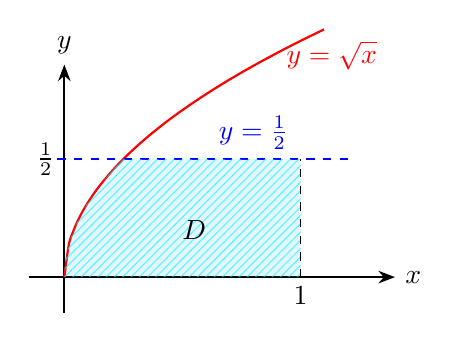
\begin{tikzpicture}[scale=3]

% Axes
\draw[-{Stealth[length=6pt]}, thick] (-0.15,0) -- (1.4,0) node[right] {$x$};
\draw[-{Stealth[length=6pt]}, thick] (0,-0.15) -- (0,0.9) node[above] {$y$};

% Curve y = sqrt(x), i.e., x = y^2
\draw[thick, red, domain=0:1.1, samples=60, smooth]
  plot (\x, {sqrt(\x)});

% Line y = 1/2
\draw[thick, blue, dashed, domain=-0.1:1.2] plot (\x, 0.5);

% Fill region D: y^2 <= x <= 1, 0 <= y <= 1/2
\fill[pattern=north east lines, pattern color=cyan, opacity=0.6]
  plot[domain=0:0.5, samples=40, smooth] ({(\x)*(\x)}, \x)
  -- (1,0.5) -- (1,0) -- (0,0) -- cycle;
\fill[cyan, opacity=0.1]
  plot[domain=0:0.5, samples=40, smooth] ({(\x)*(\x)}, \x)
  -- (1,0.5) -- (1,0) -- (0,0) -- cycle;

% Labels
\node[below] at (1,0) {$1$};
\node[left] at (0,0.5) {$\frac{1}{2}$};
\node[above right, red] at (0.9, {sqrt(0.7)}) {$y = \sqrt{x}$};
\node[above, blue] at (0.8,0.5) {$y = \frac{1}{2}$};
\node at (0.55,0.2) {$D$};

% Dashed line x=1
\draw[dashed, thin] (1,0) -- (1,0.5);

\end{tikzpicture}
\end{document}
